\chapter{Dynamic Programming}\label{chp:dynamic_programming}

% \lipsum[100]
% \blindtext[10]



The word \textbf{Dynamic} in Dynamic Programming refers that our computation complexity for the given problem can be reduced if:

\begin{enumerate}[(i)]
    \item Current state of the problem depends upon previous state solved.
    \item previous state has been already precomputed \& we have also saved their state.
\end{enumerate}


As we know recursion is way, in which current problem can be expressed in term of smaller sub-problem. Hence, writing the current state of problem in recursive way is the main step in solving question by dynamic programming.

\vspace{5mm}
% \addvspace{10cm}
Steps to Solve Dynamic Programming Question:
\begin{enumerate}[(i)]
    \itemsep0em 
    \item Express the current state of problem in recurrance relation.
    \item solve the problem in recursive way. (by considering all the edge case).
    \item Compute time complexity of recursive solution. Then compute time complexity of memoized solution.
    \item If memoized time complexiy is okay $\Rightarrow$ this is the solution.
    \item If memoized time compleixy is not okay $\Rightarrow$ express solution in alternative recurrance (same as modifying the recursive function defination) way; such that less variable term are mentioned in the recurrance relation.
\end{enumerate}

\section{Dynamic Programming Questions}
\paragraph{type1} We will list \& discuss some of the common question pattern from this paradigm.


\subsection{Classic Dynamic Problems}

\begin{problem}{0/1 Knapsack}
    We are given N items where each item has some weight and profit associated with it. We are also given a bag with capacity W, [i.e., the bag can hold at most W weight in it]. The target is to put the items into the bag such that the sum of profits associated with them is the maximum possible. 
\end{problem}

\begin{solution}
    Try thinking in term of findAns(..) function.\\

    findAns(n,w,const arr) :: maximum profit associated when we have n items \& bag with capacity w.\\
   
    % //TO-DO: Make new environment to display them side by side
    Solution1:
    \begin{verbatim}
       int findAns(int n,int w,const vector<int>& arr)
       {
            if(w<=0) return INF; //invalid case, bag capacity must always be +v
            if(n<=0) return 0; //there is no item to chose from
           

            int inc = arr[n] + findAns(n-1,w-arr[w],arr);
            int exc =  findAns(n-1,w,arr);

            return max(inc,exc);
       }
    \end{verbatim}

way2: Process element from end.
    \begin{verbatim}
        int findAns(int idx, int w, const vector<int> &arr)
        {
            if(w <= 0) return INF;
            if(idx >= arr.size()) return 0;
            

            int inc = arr[idx] + findAns(idx+1,w-arr[idx],arr);
            int exc = findAnsans(idx+1,w-arr[idx],arr);
            
            return max(inc,exc);
        }
    \end{verbatim}

way3:(preferred) best for debugging \& visualization.

    \begin{verbatim}
        int findAns(int idx,int cw,const vector<int> &arr,const int W)
        {
            if(cw > W) return INVALID; //IMP: invalid case before valid case
            if(idx >= size) return 0;
           

            int inc = arr[idx] + findAns(idx+1,cw + arr[idx], arr,W);
            int exc = findAns(idx+1,cw,arr,W);

            printf("[%d,%d] : VAL(%d,%d)\n",idx,arr[idx],inc,exc);
            return max(inc,exc);
        }
    \end{verbatim}

Issue: you need to make sure inc does not get out of bound. You can do it in various way.


\begin{enumerate}[(i)]
    \item Instead of setting INVALID as INTMAX, set it as INTMAX/2.
    \item Instead of setting as extream large value. Set it to to some large value from question constrain. This way overflow can be avoided + you get your our INF for the given question.
\end{enumerate} 


way4:(preferred) Handling Invlaid cases during call itself (Hence, no need to handling invalid cases in base-case)

    \begin{verbatim}
        int findAns(int idx,int cw, const vector<int>& arr,int W)
        {
            if(idx >= 0) return 0;

            int inc = INVALID,exc = INVALID;

            if(cw + arr[idx] <= W)
                inc = arr[idx] + findAns(idx+1,cw+arr[idx],arr,W);
            
            exc = findAns(idx+1,cw,arr,W);

            printf("[%d,%d] : VAL(%d,%d)\n",idx,arr[idx],inc,exc);
            return max(inc,exc);
        }
    \end{verbatim}

    \paragraph{Summary Of Solutions:} All of the way written above shows same logic but implemented in different way.
    way3 and way4 produces good code which is easy to debug.
    Both is preferred way, if there are more decision making at current idx, then ideally way4 is preferred. (as you can see and modify all the decision at this step itself.)

\end{solution}
\begin{problem}{Coin Change}
    Given an integer array of coins[ ] of size N representing different types of currency and an integer sum, The task is to find the number of ways to make sum by using different combinations from coins[].
\end{problem}

\begin{solution}

    let f(idx,sum) :: number of ways to make sum with [0..idx] coin from the array.

    At index idx, we have two choice:
    (a) chose the current coin
    (b) do not chose the current coin
    
    \vspace{2mm}
    Recurrance Relation: $f(idx,sum) = f(idx,sum+arr[idx]) + f(idx+1,sum)$;

    Base Case: $idx >= 0 ,sum == SUM , sum > SUM$;

    \begin{verbatim}
        int findAns(int idx, int sum,const vector<int>& arr,const int SUM)
        {
            if(sum == SUM) return 1; //for current combination 1 SUM
            if(idx >= size) return 0; //no element => no way to make SUM
            if(sum > SUM) return 0;

            int inc = findAns(idx,sum+arr[idx],arr,SUM);
            int exc = findAns(idx+1,sum,arr,SUM);

            return inc + exc;
        }
    \end{verbatim}
  
\end{solution}
\begin{problem} {Rod-Cutting}
    Given a rod of length n inches and a
table of prices pi for i= 1,2,3...i determine the maximum revenue obtainable by cutting up the rod and selling the pieces. Note that if the price pn for a rod
of length n is large enough, an optimal solution may require no cutting at all.
\end{problem}

\marginnote{
    MarginNotes
}

\begin{solution}
    (1)
    \vspace{3mm}
    \hrule
    
    \begin{intution}
        Similarity to unbounded knapsack if we consider the solution array(sarr) derived from cost[].
    \end{intution}

        % 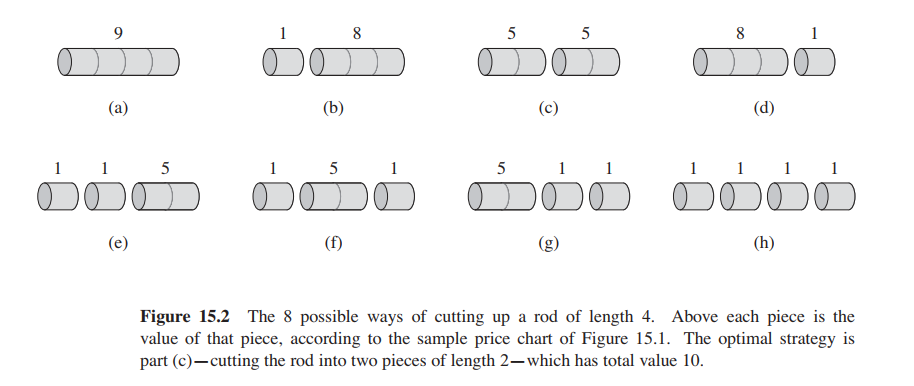
\includegraphics[width=10cm, height=5cm]{./diagram/rod-cutting-example.png}
        
       Considering the cost[], we will try to find sarr[]. \\
       where sarr[idx] := maximum revenue we can get if we are allowed to cut rod from length cost[0..idx-1]
       Now, for the sarr[] at index idx.
       We have two options:
        \begin{enumerate}[(a)]
            \item get the profit arr[idx] $\Rightarrow$ we can again cut the reduced rod with profit arr[idx] $val1 = cost[idx] + f(idx,n-(idx+1))$
            \item do not get the profit arr[idx] $val2 = f(idx+1,n)$
        \end{enumerate}
    \begin{verbatim}
        int findAns(int idx,int n ,const vector<int>& arr)
        {
            if(idx >= arr.size()) return 0;
            
            int val1 = INF; //inclusive : keep getting profit arr[idx] if its possible
            
            int val2 = INF; //exclusive: do not get profit arr[idx]
            
            int cut_length = idx+1;
            if(n-cut_length>=0)
                val1 = arr[idx] + findAns(idx,n-cut_length,arr); //rod-lenght is reduced
                
            val2 = findAns(idx+1,n,arr); 
            
            printf("[%d,%d]: (%d,%d)\n",idx,n,val1,val2);
            return max(val1,val2);
        }
    \end{verbatim}
\end{solution}


\begin{solution}
    (2)
    \vspace{3mm}
    \hrule
    
    \begin{intution}
        Consider the function signature as :
        $f(n) :=$ maximum revenu we can make if we have a rod of lenght n
    \end{intution}

    If we have rod of lenght n, that we can do cost.size() number of operations on this rod. (i.e we will try to cut this at all possible place)

    \begin{verbatim}
        int findAnsTwo(int n,const vector<int>& arr)
        {
            if(n<=0) return 0;
            int &mans = memt[n];
            if(mans != -1) return mans;

            int profit = INF;
            /* try to cut the rod in all possible way := cut the rod at 1,
            cut the rod at 2, ...
            */
            for(int k=1;k<=n;k++) //
            {
                int tprofit = arr[k-1] + findAnsTwo(n-k,arr); 
                /* question has 1 based index , so we do arr[k-1]*/
                profit = max(profit,tprofit);
            }

            return mans = profit;
        }
    \end{verbatim}
    
\end{solution}

% sol_file: /code/rod-cutting.cpp
